\documentclass{article}
\pdfpagewidth=8.5in
\pdfpageheight=11in

\usepackage{ISRreport}
\usepackage{times}
\usepackage{url}
\usepackage{xcolor}
\usepackage{polski}
\usepackage[polish]{babel}
\usepackage[utf8]{inputenc}
\usepackage[T1]{fontenc}
\usepackage[utf8]{luainputenc}
\usepackage[hidelinks]{hyperref}
\usepackage[utf8]{inputenc}

%%% fix for \lll
\let\babellll\lll
\let\lll\relax

\usepackage{amssymb}
\usepackage{amsmath}
\usepackage{caption}
\usepackage{indentfirst}
\usepackage{graphicx}
\usepackage{amsmath}
\usepackage{siunitx}
\usepackage{booktabs}
\usepackage{subfig}
\usepackage{pgfplots}
\usepackage{paracol}
\usepackage{gensymb}

\urlstyle{same}
	
\title{Inteligentne Systemy Robotyczne \\ Zadanie magazynowania sześcianów}

\author{
Jakub Sikora
\affiliations
numer albumu: 283418 \\
\emails
jakub.sikora2.stud@pw.edu.pl
}

\newcommand{\todo}[1]{\textcolor{red}{\textbf{TO DO:} #1}}

\begin{document}
\maketitle

\section{Opis problemu}
\label{sec:opis-problemu}
\subsection{Treść zadania}
\label{subsec:polecenie}
Należy zaprojektować system sterowania manipulatorem o~sześciu stopniach swobody, wyposażony w~chwytak dwustanowy oraz kamerę RGB-D (Kinect). Na taśmociągu poruszają się różnokolorowe sześciany o~wymiarach 4cm~$\pm$~1cm. Zadaniem robota jest pobieranie żółtych sześcianów poruszających się na czarnym taśmociągu i~układanie ich na palecie o~wymiarach 100cm~x~100cm. Sześciany mają być ustawione na~palecie w~konfiguracji 20x20. 

Szybkość ruchu taśmociągu jest stała i~wynosi $\num{0,1}\frac{m}{s}$ - taśmociąg nie jest sterowany przez projektowany system. Pozycja taśmociągu oraz kamery względem podstawy robota jest znana (określa je projektant systemu). Sześciany spadają pojedynczo na początek taśmociągu co 40~sekund. Ich położenie początkowe i~orientacja są losowe. Szerokość taśmociągu wynosi $\num{0.3}$ m, a~jego długość $\num{1,2}$ m. System rozpoczyna pracę po otrzymaniu komendy \texttt{START}, a~kończy ją gdy paleta się zapełni. Komendy \texttt{START} wydawane są przez zdalnego agenta, którego definiować nie potrzeba. Wymiana palet jest zadaniem innych urządzeń, które nie są pod kontrolą projektowanego systemu.

Stosująć formalizm przedstawiony na wykładzie należy:
\begin{itemize}
    \item określić strukturę systemu w~kategoriach agentów,
    \item dla każdego agenta należy zdefiniować podsystem sterowania, efektory i~receptory wirtualne,
    \item dla tych podsystemów określić:
    \begin{itemize}
        \item automat skończony sterujący ich pracą,
        \item zachowania,
        \item warunki początkowe i~końcowe zachowań,
        \item funkcje przejścia w~postaci matematycznej i~DFD,
        \item zawartość pamięci wewnętrznej oraz buforów wejściowych i~wyjściowych,
        \item krok dyskretyzacji dla każdego podsystemu.
    \end{itemize}
\end{itemize}


\section{Struktura systemu}
\label{sec:struktura}
\subsection{Konfiguracja rzeczywista}
\label{subsec:konfiguracja-urzadzen}

\begin{figure}
    \centering
    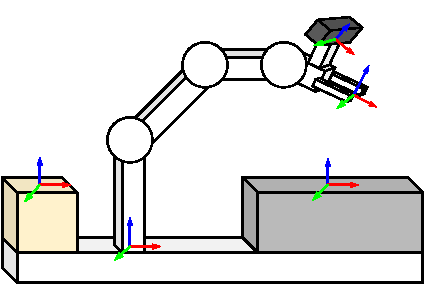
\includegraphics[width=\columnwidth]{figures/ISR-system-overview.pdf}
    \label{fig:srodowisko-robocze}
    \caption{Środowisko robocze projektowanego systemu}
\end{figure}

\subsection{Agentowa struktura systemu}
\label{subsec:agentowa-struktura}

\begin{figure}
    \centering
    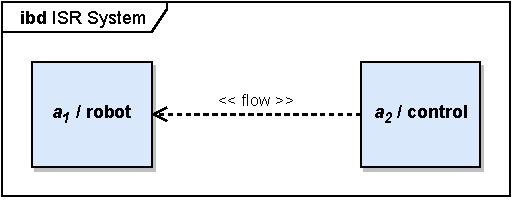
\includegraphics[width=\columnwidth]{figures/ISR-agents.pdf}
    \label{fig:agenty-system}
    \caption{Dekompozycja systemu na agenty}
\end{figure}

\begin{figure}
    \centering
    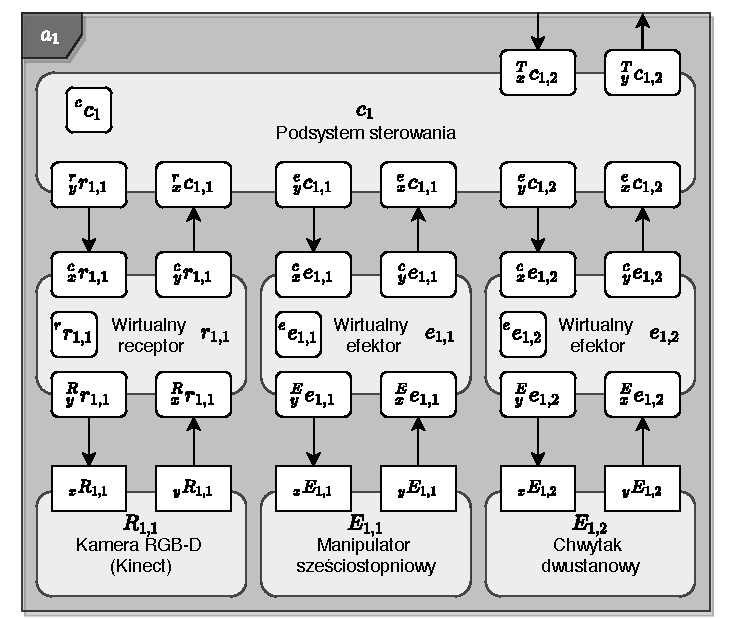
\includegraphics[width=\columnwidth]{figures/ISR-agent-decomposition.pdf}
    \label{fig:dekompozycja-agent-1}
    \caption{Dekompozycja agenta $a_{1}$ na wirtualne i~rzeczywiste receptory i~efektory}
\end{figure}


\todo{Określić niezbędne efektory oraz receptory} \\
Efektory: 
\begin{itemize}
    \item sześciostopniowy manipulator,
    \item chwytak dwustanowy.
\end{itemize}

Receptory:
\begin{itemize}
    \item kamera RGB-D.
\end{itemize}

\todo{Określić liczbę agentów przyporządkowując im efektory i
receptory (wziąć pod uwagę opóźnienia transmisyjne oraz
niezbędną moc obliczeniową)}

Z~faktu iż manipulator jest sześciostopniowy, sterowanie nim nie jest trudne (jest zawsze jedno rozwiązanie problemu kinematyki odwrotnej). Podobnie chwytak dwustanowy, jest albo zamykany albo otwierany więc też lajtowe. Największy problem to kamera RGB-D i analizowanie obrazu. Obraz Kinecta jest w niskiej rozdzielczości 640 x 480 pikseli przy 30 klatkach na sekundę. Przy 30 klatkach na sekundę, przedmioty na taśmociągu przesuną się o 3mm pomiędzy klatkami. Kamera jest umieszczona nad chwytakiem, podobnie jak w~przykładzie, kamera EIH (\emph{eye in hand}).

\todo{Określić zachowania każdego z agentów}

Podejrzewam że będą takie zachowania: 
\begin{itemize}
    \item idle,
    \item szukanie sześcianu,
    \item chwytanie,
    \item odkładanie.
\end{itemize}


\todo{Zdefiniować receptory i efektory wirtualne (widoki receptorów
i efektorów oraz bufory komunikacyjne w podsystemie sterowania)}

Slajdy od 141 dalej (wyjebane w kosmos)

Podsystem sterowania (slajdy 125-135): 

\todo{Zdefiniować okres próbkowania dla każdego podsystemu}
Receptor 30 klatek na sekundę daje 33ms.

Efektor czyta wejścia co 1ms natomiast wysyła co 20ms. 

\todo{Zbudować automat skończony przełączający zachowania}

\todo{Zdefiniować warunki początkowe dla poszczególnych zachowań}

\todo{Zdefiniować funkcje przejścia i warunki końcowe dla każdego
zachowania}

\section{Podsystem sterowania}
\label{sec:struktura}
\begin{figure}
    \centering
    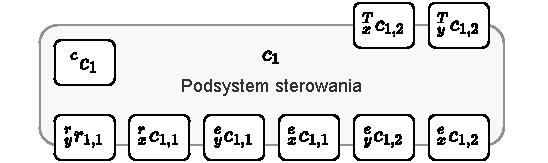
\includegraphics[width=\columnwidth]{figures/ISR-cs-model.pdf}
    \label{fig:model-cs}
    \caption{Struktura ogólna podsystemu sterowania}
\end{figure}

\begin{figure}
    \centering
    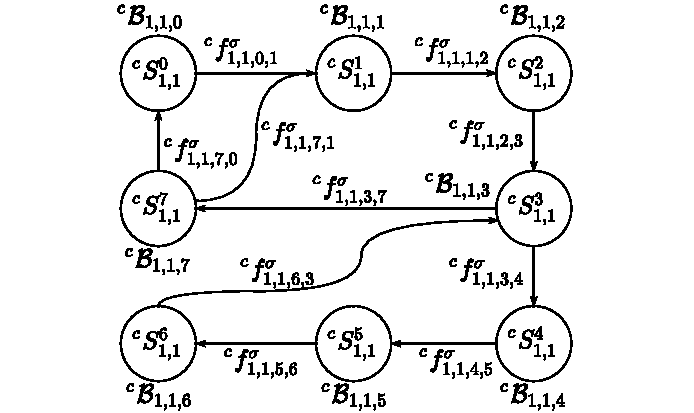
\includegraphics[width=\columnwidth]{figures/ISR-cs-behaviours.pdf}
    \label{fig:zachowania-cs}
    \caption{Automat zachowań podsystemu sterowania}
\end{figure}

Zachowania:
\begin{itemize}
    \item ${}^{c}\mathcal{B}_{1,1,0}$ - idle,
    \item ${}^{c}\mathcal{B}_{1,1,1}$ - pre-grip,
    \item ${}^{c}\mathcal{B}_{1,1,2}$ - detect-block,
    \item ${}^{c}\mathcal{B}_{1,1,3}$ - do-plan,
    \item ${}^{c}\mathcal{B}_{1,1,4}$ - grip,
    \item ${}^{c}\mathcal{B}_{1,1,5}$ - pre-store,
    \item ${}^{c}\mathcal{B}_{1,1,6}$ - detect-place,
    \item ${}^{c}\mathcal{B}_{1,1,7}$ - drop.
\end{itemize}

Bufory komunikacyjne:
\begin{itemize}
    \item ${}^{c}c_{1,1} = [g, M, \Theta_{\mathrm{plan}}, \Theta_{\mathrm{grip}}, \Theta_{\mathrm{drop}}]$ - pamięć wewnętrzna,
    
    \item ${}^{T}_{x}c_{2,1} = m \in \{ \emptyset, START \}$ - komunikat od agenta $a_{2}$,
    
    \item ${}^{r}_{y}r_{1,1} = \varphi \in \{b, p\}$ - wybór trybu pracy wirtualnego receptora kamery,
    \item ${}^{r}_{x}r_{1,1} = \Theta_{\mathrm{d}}$ - znaleziona pozycja sześcianu/miejsca w~zależności od wybranego trybu,

    \item ${}^{e}_{y}e_{1,1} = \Theta_{\mathrm{zad}}$ - zadana pozycja ramienia,
    \item ${}^{e}_{x}e_{1,1} = \Theta$ - aktualna pozycja ramienia,

    \item ${}^{e}_{y}e_{1,2} = \xi_{\mathrm{zad}} \in \{o, c\}$ - zadany stan chwytaka,
    \item ${}^{e}_{x}e_{1,2} = \Xi_{\mathrm{zad}} \in \{o, c\}$ - aktualny stan chwytaka.
\end{itemize}

Wymagane funkcje pomocnicze:
\begin{itemize}
    \item $zeros()$ - stwórz macierz 20x20 wypełnioną zerami,
    \item $isValid(\Theta)$ - sprawdza czy $\Theta$ jest poprawną pozycją,
    \item $makePlan(\Theta, \Theta_{d})$ - na podstawie aktualnego położenia, wykrytego położenia oraz znanej prędkości taśmociągu, określa położenie w~którym robot złapie sześcian, 
    \item $isFull(M)$ - sprawdza czy podana macierz zajętości palety jest wypełniona.
\end{itemize}

Warunki początkowe:
\begin{itemize}
    \item ${}^{c}f^{\sigma}_{1,1,0,1} \triangleq {}^{T}_{x}c_{2,1} = START$,
    \item ${}^{c}f^{\sigma}_{1,1,1,2} \triangleq {}^{c}f^{\tau}_{1,1,1} = True$,
    \item ${}^{c}f^{\sigma}_{1,1,2,3} \triangleq isValid(\Theta_{\mathrm{d}}) = True$,
    \item ${}^{c}f^{\sigma}_{1,1,3,1} \triangleq {}^{c}f^{\varepsilon}_{1,1,3} = True$,
    \item ${}^{c}f^{\sigma}_{1,1,3,4} \triangleq g = True$,
    \item ${}^{c}f^{\sigma}_{1,1,4,5} \triangleq {}^{c}f^{\tau}_{1,1,4} = True$,
    \item ${}^{c}f^{\sigma}_{1,1,5,6} \triangleq isValid(\Theta_{\mathrm{d}}) = True$,
    \item ${}^{c}f^{\sigma}_{1,1,6,0} \triangleq ({}^{c}f^{\tau}_{1,1,6} = True) \land (isFull(M) = False)$,
    \item ${}^{c}f^{\sigma}_{1,1,6,1} \triangleq ({}^{c}f^{\tau}_{1,1,6} = True) \land (isFull(M) = True)$,
\end{itemize}

Warunki końcowe:
\begin{itemize}
    \item ${}^{c}f^{\tau}_{1,1,0} \triangleq {}^{T}_{x}c_{2,1} = START $,
    \item ${}^{c}f^{\tau}_{1,1,1} \triangleq \Theta = \Theta_{\mathrm{grip}}$,
    \item ${}^{c}f^{\tau}_{1,1,2} \triangleq isValid(\Theta_{\mathrm{d}})$,
    \item ${}^{c}f^{\tau}_{1,1,3} \triangleq g = True$,
    \item ${}^{c}f^{\varepsilon}_{1,1,3} \triangleq g = False \land isValid(\Theta_{\mathrm{d}})$,
    \item ${}^{c}f^{\tau}_{1,1,4} \triangleq \Theta = \Theta_{\mathrm{drop}}$,
    \item ${}^{c}f^{\tau}_{1,1,5} \triangleq \Theta = \Theta_{\mathrm{d}}$,
    \item ${}^{c}f^{\tau}_{1,1,6} \triangleq g = False$,
\end{itemize}

Funkcje przejścia w postaci matematycznej:
\begin{itemize}
    \item \textbf{idle} \begin{itemize}
        \item ${}^{c_{1,1}, c_{1,1}}f_{1,1,0} \triangleq {}^{c}c_{1,1} = [False,~zeros(),~\Theta_{\mathrm{grip}},~\Theta_{\mathrm{drop}}]$,
    \end{itemize} 

    \item \textbf{pre-grip} \begin{itemize}
        \item ${}^{c_{1,1}, e_{1,1}}f_{1,1,1} \triangleq {}^{e}_{y}c_{1,1} = \Theta_{\mathrm{grip}}$
    \end{itemize}

    \item \textbf{detect-block} \begin{itemize}
        \item ${}^{c_{1,1}, r_{1,1}}f_{1,1,2} \triangleq {}^{r}_{y}c_{1,1} = b$
        \item $\Theta_{\mathrm{plan}} \triangleq 
            \begin{cases}
			    makePlan(\Theta, \Theta_{\mathrm{d}}), & isValid(\Theta_{\mathrm{d}})\\
                \emptyset, & \text{w p.p.}
		    \end{cases}$
    \end{itemize}
    
    \item \textbf{grip} \begin{itemize}
        \item ${}^{c_{1,1}, e_{1,1}}f_{1,1,3} \triangleq {}^{e}_{y}c_{1,1} = \Theta_{\mathrm{plan}}$
        \item ${}^{c_{1,1}, e_{1,2}}f_{1,1,3} \triangleq {}^{e}_{y}c_{1,2} = $
    \end{itemize}


    \item \textbf{pre-drop} \begin{itemize}
        \item ${}^{c_{1,1}, e_{1,1}}f_{1,1,0} \triangleq {}^{e}_{y}c_{1,1} = \Theta_{\mathrm{grip}}$
    \end{itemize}
    \item \textbf{detect-place} \begin{itemize}
        \item ${}^{c_{1,1}, e_{1,1}}f_{1,1,0} \triangleq {}^{e}_{y}c_{1,1} = \Theta_{\mathrm{grip}}$
    \end{itemize}
    \item \textbf{drop} \begin{itemize}
        \item ${}^{c_{1,1}, e_{1,1}}f_{1,1,0} \triangleq {}^{e}_{y}c_{1,1} = \Theta_{\mathrm{grip}}$
    \end{itemize}
\end{itemize}


\section{Wirtualny efektor manipulatora}
\label{sec:struktura}
\begin{figure}
    \centering
    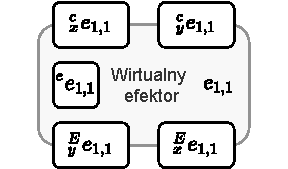
\includegraphics[width=0.75\columnwidth]{figures/ISR-ve-manip-model.pdf}
    \label{fig:model-vr-camera}
    \caption{Struktura ogólna wirtualnego efektora manipulatora sześciostopniowego}
\end{figure}

\begin{figure}
    \centering
    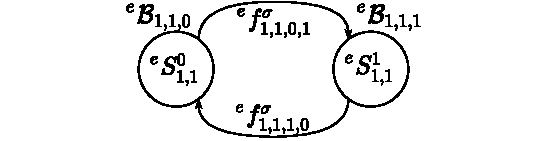
\includegraphics[width=\columnwidth]{figures/ISR-ve-manip-behaviours.pdf}
    \label{fig:zachowania-ve-manip}
    \caption{Automat zachowań wirtualnego efektora manipulatora sześciostopniowego}
\end{figure}

Efektor wirtualny manipulatora:
\begin{itemize}
    \item bufor wejściowy od podsystemu sterowania: pozycja pożądana,
    \item bufor wyjściowy do podsystemu sterowania: pozycja aktualna,
    \item bufor wejściowy od rzeczywistego efektora: aktualne położenie wałów silnika,
    \item bufor wyjściowy do rzeczywistego efektora: pożądana pozycja wałów silnika.
\end{itemize}


Zachowania:
\begin{itemize}
    \item ${}^{e}\mathcal{B}_{1,1,0}$ - idle,
    \item ${}^{e}\mathcal{B}_{1,1,1}$ - move.
\end{itemize}

\section{Wirtualny efektor chwytaka}
\label{sec:struktura}
\subsection{Struktura wirtualnego efektora}
\label{subsec:ve-gripper-struktura}

\begin{figure}[ht]
    \centering
    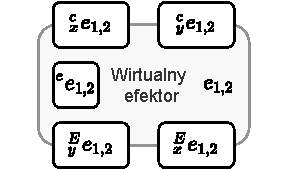
\includegraphics[width=0.75\columnwidth]{figures/ISR-ve-gripper-model.pdf}
    \caption{Struktura ogólna wirtualnego efektora chwytaka dwustanowego}
    \label{fig:model-ve-gripper}
\end{figure}

Na rysunku~\ref{fig:model-ve-gripper} przedstawiono widok wirtualnego efektora chwytaka dwustanowego w~projektowanym systemie. Jego rolą jest nadzorowanie pracą rzeczywistego efektora sterującego chwytakiem. Do poprawnej pracy podsystemu wymagane są wszystkie cztery bufory komunikacyjne, jednak nie potrzebuje on do działania wewnętrznej pamięci. Podobnie jak efektor manipulatora, krok dyskretyzacji został ustawiony na ${}^{e}T = \frac{1}{30}s$.

\subsubsection{Bufory komunikacyjne}
\begin{itemize}
    \item ${}^{c}_{x}e_{1,2} = \xi_{\mathrm{zad}} \in \{o, c\}$ - zadany stan chwytaka,
    \item ${}^{c}_{y}e_{1,2} = \xi \in \{o, c\}$ - aktualny stan chwytaka przesyłany do podsystemu sterowania,
    \item ${}^{E}_{x}e_{1,2} = \Xi \in \{o, c\}$ - aktualny stan chwytaka, aktualizowany po pełnym rozwarciu chwytaka lub po maksymalnym domknięciu,
    \item ${}^{E}_{y}e_{1,2} = \Xi_{\mathrm{zad}} \in \{o, c\}$ - aktualnie realizowany stan chwytaka.
\end{itemize}

\subsection{Automat sterujący}
Prostota działania chwytaka implikuje jeden stan normalnej pracy urządzenia, z~którym skojarzone zostało zachowanie ${}^{e}\mathcal{B}_{1,2,0}$ (\textbf{work}). Zachowanie \textbf{work} jest jedynym zachowaniem podsystemu, dlatego nie ma potrzeby rozważania warunków początkowych oraz końcowych. 

\subsubsection{Funkcja przejścia}
\begin{equation}
    \begin{gathered}
        {}^{e_{1,2}, E_{1,2}}f_{1,2,0} \triangleq {}^{E}_{y}e_{1,2} = \xi,\\
        {}^{e_{1,2}, c_{1,1}}f_{1,2,0} \triangleq {}^{c}_{y}e_{1,2} = \Xi
    \end{gathered}
\end{equation}

\begin{figure}
    \centering
    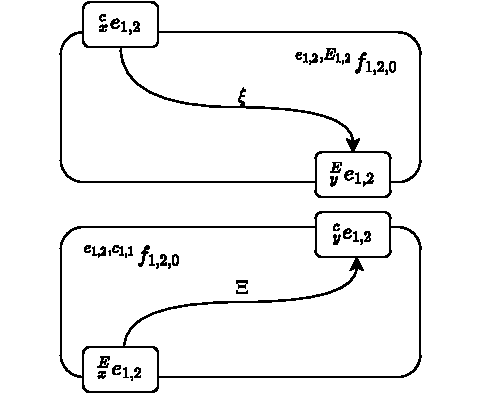
\includegraphics[width=\columnwidth]{figures/ISR-ve-gripper-fp-work.pdf}
    \label{fig:ve-gripper-fp-work}
    \caption{Zdekomponowana funkcja przejścia zachowania \textbf{work} w~postaci DFD}
\end{figure}


%%%%%%%%%%%%%%%%%%%%%%%%%%%%%%%%%%%%%%%%%%%%%%%%%%%%%%%%%%%%%%%%%%%%%%%%%%%%%%%%%

\section{Wirtualny receptor kamery RGB-D}
\label{sec:struktura}
\subsection{Struktura wirtualnego receptora}
\label{subsec:vr-camera-struktura}

\begin{figure}[ht]
    \centering
    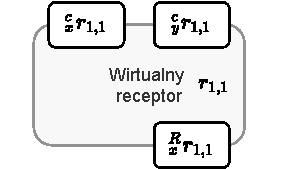
\includegraphics[width=0.75\columnwidth]{figures/ISR-vr-camera-model.pdf}
    \caption{Struktura ogólna wirtualnego receptora kamery RGB-D}
    \label{fig:model-vr-camera}
\end{figure}

Na rysunku~\ref{fig:model-vr-camera} przedstawiono strukturę wirtualnego receptora. Jego rolą jest odbiór surowych danych pomiarowych z~rzeczywistego receptora oraz ich obróbka i~agregacja przed wysłaniem ich do podsystemu sterowania. Do poprawnej pracy podsystemu, wymagane są trzy bufory komunikacyjne: dwa do komunikacji z~podsystemem sterowania oraz jeden do odbioru danych z~kamery. Krok dyskretyzacji wirtualnego receptora jest wąskim gardłem systemu. Założono że receptor jest w~stanie działać z krokiem ${}^{r}T = \frac{1}{30}$s, czyli takim z~jakim działa wirtualny receptor. Założenie to jest wykonalne z~racji niskiej rozdzielczości kamer tego typu.

\subsubsection{Bufory komunikacyjne}
\begin{itemize}
    \item ${}^{c}_{x}r_{1,1} = \varphi \in \{b, p\}$ - tryb detekcji klocków/miejsc,
    \item ${}^{c}_{y}r_{1,1} = \Theta_{d}$ - pozycja wykrywanego klocka/miejsca,
    \item ${}^{R}_{x}r_{1,1} = \Lambda$ - chmura punktów z~kamery RGB-D.
\end{itemize}

\subsubsection{Funkcje pomocnicze}
Do poprawnego działania receptora, wymagana jest implementacja kilku funkcji pomocniczych, których konkretna definicja wymaga dokładnych parametrów omawianej kamery oraz budowy palety. Ich nagłówki zostały ograniczone do minimum, tak aby przedstawić ideę przetwarzania w~podsystemie.

\begin{itemize}
    \item \texttt{detect($\Lambda$)} - wykryj żółty sześciany
    \item \texttt{getTF($c$)} - zwróć pozycję podanego sześcianu,
    
    \item \texttt{find($\Lambda$)} - wykryj możliwe położenia do odstawienia,
    \item \texttt{getFinal($s$)} - zwróć pozycję docelowych położeń do odstawienia sześcianu, wraz z~ich koordynatami na palecie.
\end{itemize}

\subsection{Automat sterujący}
\begin{figure}[ht]
    \centering
    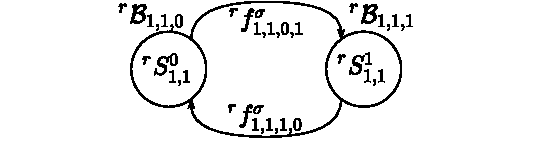
\includegraphics[width=\columnwidth]{figures/ISR-vr-camera-behaviours.pdf}
    \caption{Automat zachowań wirtualnego receptora kamery RGB-D}
    \label{fig:zachowania-vr-camera}
\end{figure}


Na rysunku~\ref{fig:zachowania-vr-camera} przedstawiony został automat sterujący wirtualnym receptorem kamery. Z~każdym z~dwóch stanów $ {}^{r}S_{1,1}^0,  {}^{r}S_{1,1}^1$ skojarzone zostało zachowanie ${}^{r}\mathcal{B}_{1,1,0}$ (\textbf{blocks}) oraz ${}^{r}\mathcal{B}_{1,1,1}$ (\textbf{places}). Każde z~zachowań określa tryb przetwarzania danych z~kamery. Wybór zachowań następuje poprzez wysłanie odpowiedniej wartości na bufor wejściowy.

\subsection{Zachowanie blocks}
\label{subsec:vr-camera-blocks}
Zachowanie ${}^{r}\mathcal{B}_{1,1,0}$ określa tryb wykrywania żółtych sześcianów. Gdy to zachowanie jest aktywne, na bufor ${}^{c}_{y}r_{1,1} = \Theta_{d}$ wysyłana jest pozycja wykrytego klocka lub wartość pusta. 

\subsubsection{Funkcja przejścia}
\begin{equation}
    {}^{r_{1,1}, c_{1,1}}f_{1,1,0} \triangleq {}^{c}_{y}e_{1,1} = \text{\texttt{getTF(detect(}}\Lambda\text{\texttt{))}}    
\end{equation}

\begin{figure}[ht]
    \centering
    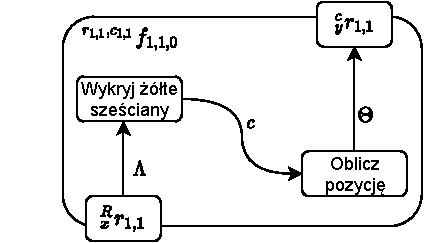
\includegraphics[width=\columnwidth]{figures/ISR-vr-camera-fp-blocks.pdf}
    \label{fig:vr-camera-fp-blocks}
    \caption{Zdekomponowana funkcja przejścia zachowania \textbf{blocks} w~postaci DFD}
\end{figure}

\subsubsection{Warunki początkowe}
\begin{equation}
    {}^{r}f^{\sigma}_{1,1,1,0} \triangleq \varphi = b
\end{equation}

\subsubsection{Warunki końcowe}
\begin{equation}
    {}^{r}f^{\tau}_{1,1,0} \triangleq \varphi \neq b
\end{equation}

\subsection{Zachowanie places}
\label{subsec:vr-camera-places}
Zachowanie ${}^{r}\mathcal{B}_{1,1,1}$ określa tryb wykrywania miejsc na palecie. Gdy to zachowanie jest aktywne, na bufor ${}^{c}_{y}r_{1,1} = \Theta_{d}$ wysyłana jest lista dostępnych pozycji wraz z~ich koordynatami na palecie lub wartość pusta. 

\subsubsection{Funkcja przejścia}
\begin{equation}
    {}^{r_{1,1}, c_{1,1}}f_{1,1,1} \triangleq {}^{c}_{y}e_{1,1} = \text{\texttt{getFinal(find(}}\Lambda\text{\texttt{))}}  
\end{equation}

\begin{figure}[ht]
    \centering
    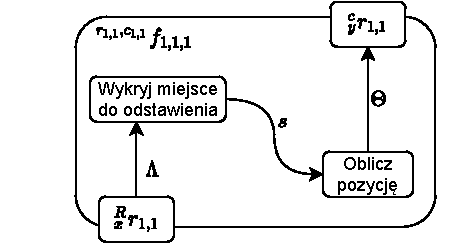
\includegraphics[width=\columnwidth]{figures/ISR-vr-camera-fp-places.pdf}
    \label{fig:vr-camera-fp-places}
    \caption{Zdekomponowana funkcja przejścia zachowania \textbf{places} w~postaci DFD}
\end{figure}

\subsubsection{Warunki początkowe}
\begin{equation}
    {}^{r}f^{\sigma}_{1,1,1,0} \triangleq \varphi = p
\end{equation}

\subsubsection{Warunki końcowe}
\begin{equation}
    {}^{r}f^{\tau}_{1,1,0} \triangleq \varphi \neq p
\end{equation}



\bibliographystyle{abbrv}
\bibliography{bibliography}

\end{document}